\documentclass[a4paper]{article}
\usepackage{pgfplots}
\usepackage{pgfplotstable}
\pgfplotsset{width=7cm,compat=1.13}
\begin{document}
	
	
	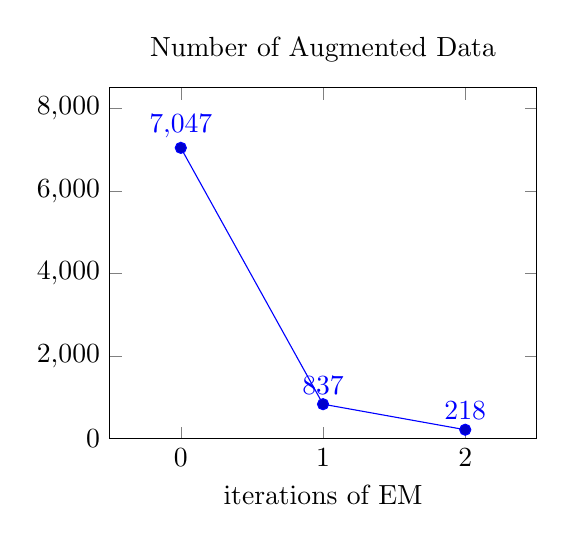
\begin{tikzpicture}
		\begin{axis}
			[
			legend pos=outer north east,  % 将图例放在图外,位于图的东北角
			xlabel=iterations of EM,
			title=Number of Augmented Data,
			ymax=8500,
			ymin=0,
			xmin=-0.5,
			xmax=2.5,
			nodes near coords={\pgfmathprintnumber{\pgfkeysvalueof{/data point/y}}},
			]
			\addplot 
			table                               % 绘制原始数据的折线图
			{           		                % X,Y的原始数据
				X Y
				0 7047
				1 837
				2 218
			};
		\end{axis}
	\end{tikzpicture}
	
	
	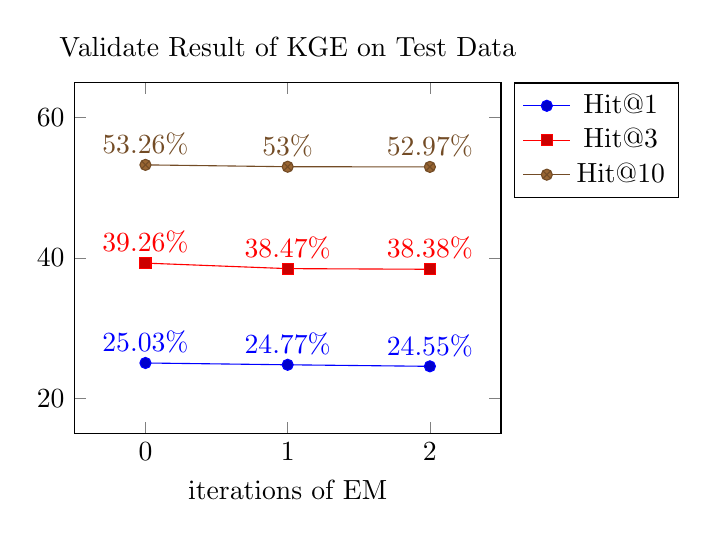
\begin{tikzpicture}
		\begin{axis}
			[
				legend pos=outer north east,
				xlabel=iterations of EM,
				title=Validate Result of KGE on Test Data,
				ymax=65,
				ymin=15,
				xmin=-0.5,
				xmax=2.5,
				nodes near coords={\pgfmathprintnumber{\pgfkeysvalueof{/data point/y}}\%},
			]
			\addplot 
			table                               % 绘制原始数据的折线图
			{           		                % X,Y的原始数据
				X Y
				0 25.0264
				1 24.7693
				2 24.5499
			};
			\addplot
			table
			% table[y={create col/linear regression={y=Y}}] % 对输入的数据作线性回归
			{   				
				X Y
				0 39.2603
				1 38.4737
				2 38.3829
			};
			\addplot
			table
			{   				
				X Y
				0 53.2597
				1 52.9950
				2 52.9723
			};
			\addlegendentry{Hit@1}          % 给第一个图像添加图例,即原始函数y(x)
			\addlegendentry{Hit@3}          % 给第一个图像添加图例,即原始函数y(x)
			\addlegendentry{Hit@10}          % 给第一个图像添加图例,即原始函数y(x)

			% \addlegendentry{                 % 给第二个图像添加图例,即线性回归结果a*x+b
			% 	$\pgfmathprintnumber{\pgfplotstableregressiona} \cdot x
			% 	\pgfmathprintnumber[print sign]{\pgfplotstableregressionb}$}
		\end{axis}
	\end{tikzpicture}


	
	
	
	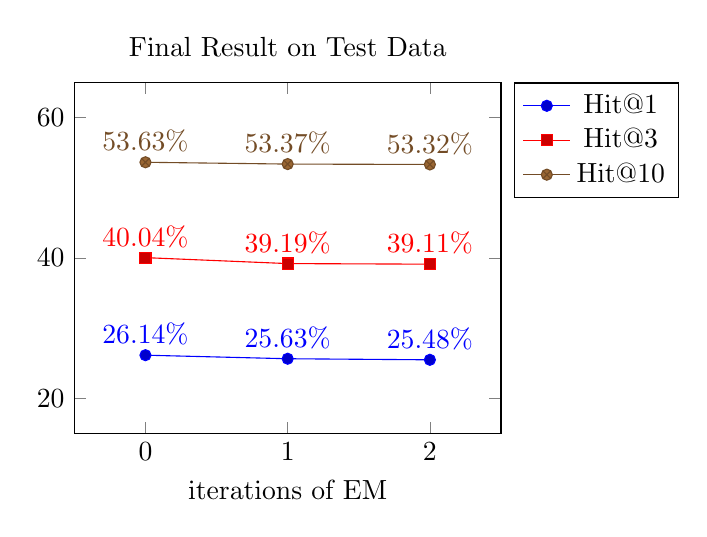
\begin{tikzpicture}
		\begin{axis}
			[
			legend pos=outer north east,
			title=Final Result on Test Data,
			xlabel=iterations of EM,
			ymax=65,
			ymin=15,
			xmin=-0.5,
			xmax=2.5,
			nodes near coords={\pgfmathprintnumber{\pgfkeysvalueof{/data point/y}}\%},
			]
			\addplot 
			table                               % 绘制原始数据的折线图
			{           		                % X,Y的原始数据
				X Y
				0 26.1382
				1 25.6315
				2 25.4802
			};
			\addplot
			table
			% table[y={create col/linear regression={y=Y}}] % 对输入的数据作线性回归
			{   				
				X Y
				0 40.0393
				1 39.1922
				2 39.1090
			};
			\addplot
			table
			{   				
				X Y
				0 53.6303
				1 53.3731
				2 53.3202
			};
			\addlegendentry{Hit@1}          % 给第一个图像添加图例,即原始函数y(x)
			\addlegendentry{Hit@3}          % 给第一个图像添加图例,即原始函数y(x)
			\addlegendentry{Hit@10}          % 给第一个图像添加图例,即原始函数y(x)
			
			% \addlegendentry{                 % 给第二个图像添加图例,即线性回归结果a*x+b
				% 	$\pgfmathprintnumber{\pgfplotstableregressiona} \cdot x
				% 	\pgfmathprintnumber[print sign]{\pgfplotstableregressionb}$}
		\end{axis}
	\end{tikzpicture}



\end{document}
